\documentclass[11pt]{article}

    \usepackage[breakable]{tcolorbox}
    \usepackage{parskip} % Stop auto-indenting (to mimic markdown behaviour)
    

    % Basic figure setup, for now with no caption control since it's done
    % automatically by Pandoc (which extracts ![](path) syntax from Markdown).
    \usepackage{graphicx}
    % Maintain compatibility with old templates. Remove in nbconvert 6.0
    \let\Oldincludegraphics\includegraphics
    % Ensure that by default, figures have no caption (until we provide a
    % proper Figure object with a Caption API and a way to capture that
    % in the conversion process - todo).
    \usepackage{caption}
    \DeclareCaptionFormat{nocaption}{}
    \captionsetup{format=nocaption,aboveskip=0pt,belowskip=0pt}

    \usepackage{float}
    \floatplacement{figure}{H} % forces figures to be placed at the correct location
    \usepackage{xcolor} % Allow colors to be defined
    \usepackage{enumerate} % Needed for markdown enumerations to work
    \usepackage{geometry} % Used to adjust the document margins
    \usepackage{amsmath} % Equations
    \usepackage{amssymb} % Equations
    \usepackage{textcomp} % defines textquotesingle
    % Hack from http://tex.stackexchange.com/a/47451/13684:
    \AtBeginDocument{%
        \def\PYZsq{\textquotesingle}% Upright quotes in Pygmentized code
    }
    \usepackage{upquote} % Upright quotes for verbatim code
    \usepackage{eurosym} % defines \euro

    \usepackage{iftex}
    \ifPDFTeX
        \usepackage[T1]{fontenc}
        \IfFileExists{alphabeta.sty}{
              \usepackage{alphabeta}
          }{
              \usepackage[mathletters]{ucs}
              \usepackage[utf8x]{inputenc}
          }
    \else
        \usepackage{fontspec}
        \usepackage{unicode-math}
    \fi

    \usepackage{fancyvrb} % verbatim replacement that allows latex
    \usepackage{grffile} % extends the file name processing of package graphics
                         % to support a larger range
    \makeatletter % fix for old versions of grffile with XeLaTeX
    \@ifpackagelater{grffile}{2019/11/01}
    {
      % Do nothing on new versions
    }
    {
      \def\Gread@@xetex#1{%
        \IfFileExists{"\Gin@base".bb}%
        {\Gread@eps{\Gin@base.bb}}%
        {\Gread@@xetex@aux#1}%
      }
    }
    \makeatother
    \usepackage[Export]{adjustbox} % Used to constrain images to a maximum size
    \adjustboxset{max size={0.9\linewidth}{0.9\paperheight}}

    % The hyperref package gives us a pdf with properly built
    % internal navigation ('pdf bookmarks' for the table of contents,
    % internal cross-reference links, web links for URLs, etc.)
    \usepackage{hyperref}
    % The default LaTeX title has an obnoxious amount of whitespace. By default,
    % titling removes some of it. It also provides customization options.
    \usepackage{titling}
    \usepackage{longtable} % longtable support required by pandoc >1.10
    \usepackage{booktabs}  % table support for pandoc > 1.12.2
    \usepackage{array}     % table support for pandoc >= 2.11.3
    \usepackage{calc}      % table minipage width calculation for pandoc >= 2.11.1
    \usepackage[inline]{enumitem} % IRkernel/repr support (it uses the enumerate* environment)
    \usepackage[normalem]{ulem} % ulem is needed to support strikethroughs (\sout)
                                % normalem makes italics be italics, not underlines
    \usepackage{mathrsfs}
    

    
    % Colors for the hyperref package
    \definecolor{urlcolor}{rgb}{0,.145,.698}
    \definecolor{linkcolor}{rgb}{.71,0.21,0.01}
    \definecolor{citecolor}{rgb}{.12,.54,.11}

    % ANSI colors
    \definecolor{ansi-black}{HTML}{3E424D}
    \definecolor{ansi-black-intense}{HTML}{282C36}
    \definecolor{ansi-red}{HTML}{E75C58}
    \definecolor{ansi-red-intense}{HTML}{B22B31}
    \definecolor{ansi-green}{HTML}{00A250}
    \definecolor{ansi-green-intense}{HTML}{007427}
    \definecolor{ansi-yellow}{HTML}{DDB62B}
    \definecolor{ansi-yellow-intense}{HTML}{B27D12}
    \definecolor{ansi-blue}{HTML}{208FFB}
    \definecolor{ansi-blue-intense}{HTML}{0065CA}
    \definecolor{ansi-magenta}{HTML}{D160C4}
    \definecolor{ansi-magenta-intense}{HTML}{A03196}
    \definecolor{ansi-cyan}{HTML}{60C6C8}
    \definecolor{ansi-cyan-intense}{HTML}{258F8F}
    \definecolor{ansi-white}{HTML}{C5C1B4}
    \definecolor{ansi-white-intense}{HTML}{A1A6B2}
    \definecolor{ansi-default-inverse-fg}{HTML}{FFFFFF}
    \definecolor{ansi-default-inverse-bg}{HTML}{000000}

    % common color for the border for error outputs.
    \definecolor{outerrorbackground}{HTML}{FFDFDF}

    % commands and environments needed by pandoc snippets
    % extracted from the output of `pandoc -s`
    \providecommand{\tightlist}{%
      \setlength{\itemsep}{0pt}\setlength{\parskip}{0pt}}
    \DefineVerbatimEnvironment{Highlighting}{Verbatim}{commandchars=\\\{\}}
    % Add ',fontsize=\small' for more characters per line
    \newenvironment{Shaded}{}{}
    \newcommand{\KeywordTok}[1]{\textcolor[rgb]{0.00,0.44,0.13}{\textbf{{#1}}}}
    \newcommand{\DataTypeTok}[1]{\textcolor[rgb]{0.56,0.13,0.00}{{#1}}}
    \newcommand{\DecValTok}[1]{\textcolor[rgb]{0.25,0.63,0.44}{{#1}}}
    \newcommand{\BaseNTok}[1]{\textcolor[rgb]{0.25,0.63,0.44}{{#1}}}
    \newcommand{\FloatTok}[1]{\textcolor[rgb]{0.25,0.63,0.44}{{#1}}}
    \newcommand{\CharTok}[1]{\textcolor[rgb]{0.25,0.44,0.63}{{#1}}}
    \newcommand{\StringTok}[1]{\textcolor[rgb]{0.25,0.44,0.63}{{#1}}}
    \newcommand{\CommentTok}[1]{\textcolor[rgb]{0.38,0.63,0.69}{\textit{{#1}}}}
    \newcommand{\OtherTok}[1]{\textcolor[rgb]{0.00,0.44,0.13}{{#1}}}
    \newcommand{\AlertTok}[1]{\textcolor[rgb]{1.00,0.00,0.00}{\textbf{{#1}}}}
    \newcommand{\FunctionTok}[1]{\textcolor[rgb]{0.02,0.16,0.49}{{#1}}}
    \newcommand{\RegionMarkerTok}[1]{{#1}}
    \newcommand{\ErrorTok}[1]{\textcolor[rgb]{1.00,0.00,0.00}{\textbf{{#1}}}}
    \newcommand{\NormalTok}[1]{{#1}}

    % Additional commands for more recent versions of Pandoc
    \newcommand{\ConstantTok}[1]{\textcolor[rgb]{0.53,0.00,0.00}{{#1}}}
    \newcommand{\SpecialCharTok}[1]{\textcolor[rgb]{0.25,0.44,0.63}{{#1}}}
    \newcommand{\VerbatimStringTok}[1]{\textcolor[rgb]{0.25,0.44,0.63}{{#1}}}
    \newcommand{\SpecialStringTok}[1]{\textcolor[rgb]{0.73,0.40,0.53}{{#1}}}
    \newcommand{\ImportTok}[1]{{#1}}
    \newcommand{\DocumentationTok}[1]{\textcolor[rgb]{0.73,0.13,0.13}{\textit{{#1}}}}
    \newcommand{\AnnotationTok}[1]{\textcolor[rgb]{0.38,0.63,0.69}{\textbf{\textit{{#1}}}}}
    \newcommand{\CommentVarTok}[1]{\textcolor[rgb]{0.38,0.63,0.69}{\textbf{\textit{{#1}}}}}
    \newcommand{\VariableTok}[1]{\textcolor[rgb]{0.10,0.09,0.49}{{#1}}}
    \newcommand{\ControlFlowTok}[1]{\textcolor[rgb]{0.00,0.44,0.13}{\textbf{{#1}}}}
    \newcommand{\OperatorTok}[1]{\textcolor[rgb]{0.40,0.40,0.40}{{#1}}}
    \newcommand{\BuiltInTok}[1]{{#1}}
    \newcommand{\ExtensionTok}[1]{{#1}}
    \newcommand{\PreprocessorTok}[1]{\textcolor[rgb]{0.74,0.48,0.00}{{#1}}}
    \newcommand{\AttributeTok}[1]{\textcolor[rgb]{0.49,0.56,0.16}{{#1}}}
    \newcommand{\InformationTok}[1]{\textcolor[rgb]{0.38,0.63,0.69}{\textbf{\textit{{#1}}}}}
    \newcommand{\WarningTok}[1]{\textcolor[rgb]{0.38,0.63,0.69}{\textbf{\textit{{#1}}}}}


    % Define a nice break command that doesn't care if a line doesn't already
    % exist.
    \def\br{\hspace*{\fill} \\* }
    % Math Jax compatibility definitions
    \def\gt{>}
    \def\lt{<}
    \let\Oldtex\TeX
    \let\Oldlatex\LaTeX
    \renewcommand{\TeX}{\textrm{\Oldtex}}
    \renewcommand{\LaTeX}{\textrm{\Oldlatex}}
    % Document parameters
    % Document title
    \title{index}
    
    
    
    
    
% Pygments definitions
\makeatletter
\def\PY@reset{\let\PY@it=\relax \let\PY@bf=\relax%
    \let\PY@ul=\relax \let\PY@tc=\relax%
    \let\PY@bc=\relax \let\PY@ff=\relax}
\def\PY@tok#1{\csname PY@tok@#1\endcsname}
\def\PY@toks#1+{\ifx\relax#1\empty\else%
    \PY@tok{#1}\expandafter\PY@toks\fi}
\def\PY@do#1{\PY@bc{\PY@tc{\PY@ul{%
    \PY@it{\PY@bf{\PY@ff{#1}}}}}}}
\def\PY#1#2{\PY@reset\PY@toks#1+\relax+\PY@do{#2}}

\@namedef{PY@tok@w}{\def\PY@tc##1{\textcolor[rgb]{0.73,0.73,0.73}{##1}}}
\@namedef{PY@tok@c}{\let\PY@it=\textit\def\PY@tc##1{\textcolor[rgb]{0.24,0.48,0.48}{##1}}}
\@namedef{PY@tok@cp}{\def\PY@tc##1{\textcolor[rgb]{0.61,0.40,0.00}{##1}}}
\@namedef{PY@tok@k}{\let\PY@bf=\textbf\def\PY@tc##1{\textcolor[rgb]{0.00,0.50,0.00}{##1}}}
\@namedef{PY@tok@kp}{\def\PY@tc##1{\textcolor[rgb]{0.00,0.50,0.00}{##1}}}
\@namedef{PY@tok@kt}{\def\PY@tc##1{\textcolor[rgb]{0.69,0.00,0.25}{##1}}}
\@namedef{PY@tok@o}{\def\PY@tc##1{\textcolor[rgb]{0.40,0.40,0.40}{##1}}}
\@namedef{PY@tok@ow}{\let\PY@bf=\textbf\def\PY@tc##1{\textcolor[rgb]{0.67,0.13,1.00}{##1}}}
\@namedef{PY@tok@nb}{\def\PY@tc##1{\textcolor[rgb]{0.00,0.50,0.00}{##1}}}
\@namedef{PY@tok@nf}{\def\PY@tc##1{\textcolor[rgb]{0.00,0.00,1.00}{##1}}}
\@namedef{PY@tok@nc}{\let\PY@bf=\textbf\def\PY@tc##1{\textcolor[rgb]{0.00,0.00,1.00}{##1}}}
\@namedef{PY@tok@nn}{\let\PY@bf=\textbf\def\PY@tc##1{\textcolor[rgb]{0.00,0.00,1.00}{##1}}}
\@namedef{PY@tok@ne}{\let\PY@bf=\textbf\def\PY@tc##1{\textcolor[rgb]{0.80,0.25,0.22}{##1}}}
\@namedef{PY@tok@nv}{\def\PY@tc##1{\textcolor[rgb]{0.10,0.09,0.49}{##1}}}
\@namedef{PY@tok@no}{\def\PY@tc##1{\textcolor[rgb]{0.53,0.00,0.00}{##1}}}
\@namedef{PY@tok@nl}{\def\PY@tc##1{\textcolor[rgb]{0.46,0.46,0.00}{##1}}}
\@namedef{PY@tok@ni}{\let\PY@bf=\textbf\def\PY@tc##1{\textcolor[rgb]{0.44,0.44,0.44}{##1}}}
\@namedef{PY@tok@na}{\def\PY@tc##1{\textcolor[rgb]{0.41,0.47,0.13}{##1}}}
\@namedef{PY@tok@nt}{\let\PY@bf=\textbf\def\PY@tc##1{\textcolor[rgb]{0.00,0.50,0.00}{##1}}}
\@namedef{PY@tok@nd}{\def\PY@tc##1{\textcolor[rgb]{0.67,0.13,1.00}{##1}}}
\@namedef{PY@tok@s}{\def\PY@tc##1{\textcolor[rgb]{0.73,0.13,0.13}{##1}}}
\@namedef{PY@tok@sd}{\let\PY@it=\textit\def\PY@tc##1{\textcolor[rgb]{0.73,0.13,0.13}{##1}}}
\@namedef{PY@tok@si}{\let\PY@bf=\textbf\def\PY@tc##1{\textcolor[rgb]{0.64,0.35,0.47}{##1}}}
\@namedef{PY@tok@se}{\let\PY@bf=\textbf\def\PY@tc##1{\textcolor[rgb]{0.67,0.36,0.12}{##1}}}
\@namedef{PY@tok@sr}{\def\PY@tc##1{\textcolor[rgb]{0.64,0.35,0.47}{##1}}}
\@namedef{PY@tok@ss}{\def\PY@tc##1{\textcolor[rgb]{0.10,0.09,0.49}{##1}}}
\@namedef{PY@tok@sx}{\def\PY@tc##1{\textcolor[rgb]{0.00,0.50,0.00}{##1}}}
\@namedef{PY@tok@m}{\def\PY@tc##1{\textcolor[rgb]{0.40,0.40,0.40}{##1}}}
\@namedef{PY@tok@gh}{\let\PY@bf=\textbf\def\PY@tc##1{\textcolor[rgb]{0.00,0.00,0.50}{##1}}}
\@namedef{PY@tok@gu}{\let\PY@bf=\textbf\def\PY@tc##1{\textcolor[rgb]{0.50,0.00,0.50}{##1}}}
\@namedef{PY@tok@gd}{\def\PY@tc##1{\textcolor[rgb]{0.63,0.00,0.00}{##1}}}
\@namedef{PY@tok@gi}{\def\PY@tc##1{\textcolor[rgb]{0.00,0.52,0.00}{##1}}}
\@namedef{PY@tok@gr}{\def\PY@tc##1{\textcolor[rgb]{0.89,0.00,0.00}{##1}}}
\@namedef{PY@tok@ge}{\let\PY@it=\textit}
\@namedef{PY@tok@gs}{\let\PY@bf=\textbf}
\@namedef{PY@tok@gp}{\let\PY@bf=\textbf\def\PY@tc##1{\textcolor[rgb]{0.00,0.00,0.50}{##1}}}
\@namedef{PY@tok@go}{\def\PY@tc##1{\textcolor[rgb]{0.44,0.44,0.44}{##1}}}
\@namedef{PY@tok@gt}{\def\PY@tc##1{\textcolor[rgb]{0.00,0.27,0.87}{##1}}}
\@namedef{PY@tok@err}{\def\PY@bc##1{{\setlength{\fboxsep}{\string -\fboxrule}\fcolorbox[rgb]{1.00,0.00,0.00}{1,1,1}{\strut ##1}}}}
\@namedef{PY@tok@kc}{\let\PY@bf=\textbf\def\PY@tc##1{\textcolor[rgb]{0.00,0.50,0.00}{##1}}}
\@namedef{PY@tok@kd}{\let\PY@bf=\textbf\def\PY@tc##1{\textcolor[rgb]{0.00,0.50,0.00}{##1}}}
\@namedef{PY@tok@kn}{\let\PY@bf=\textbf\def\PY@tc##1{\textcolor[rgb]{0.00,0.50,0.00}{##1}}}
\@namedef{PY@tok@kr}{\let\PY@bf=\textbf\def\PY@tc##1{\textcolor[rgb]{0.00,0.50,0.00}{##1}}}
\@namedef{PY@tok@bp}{\def\PY@tc##1{\textcolor[rgb]{0.00,0.50,0.00}{##1}}}
\@namedef{PY@tok@fm}{\def\PY@tc##1{\textcolor[rgb]{0.00,0.00,1.00}{##1}}}
\@namedef{PY@tok@vc}{\def\PY@tc##1{\textcolor[rgb]{0.10,0.09,0.49}{##1}}}
\@namedef{PY@tok@vg}{\def\PY@tc##1{\textcolor[rgb]{0.10,0.09,0.49}{##1}}}
\@namedef{PY@tok@vi}{\def\PY@tc##1{\textcolor[rgb]{0.10,0.09,0.49}{##1}}}
\@namedef{PY@tok@vm}{\def\PY@tc##1{\textcolor[rgb]{0.10,0.09,0.49}{##1}}}
\@namedef{PY@tok@sa}{\def\PY@tc##1{\textcolor[rgb]{0.73,0.13,0.13}{##1}}}
\@namedef{PY@tok@sb}{\def\PY@tc##1{\textcolor[rgb]{0.73,0.13,0.13}{##1}}}
\@namedef{PY@tok@sc}{\def\PY@tc##1{\textcolor[rgb]{0.73,0.13,0.13}{##1}}}
\@namedef{PY@tok@dl}{\def\PY@tc##1{\textcolor[rgb]{0.73,0.13,0.13}{##1}}}
\@namedef{PY@tok@s2}{\def\PY@tc##1{\textcolor[rgb]{0.73,0.13,0.13}{##1}}}
\@namedef{PY@tok@sh}{\def\PY@tc##1{\textcolor[rgb]{0.73,0.13,0.13}{##1}}}
\@namedef{PY@tok@s1}{\def\PY@tc##1{\textcolor[rgb]{0.73,0.13,0.13}{##1}}}
\@namedef{PY@tok@mb}{\def\PY@tc##1{\textcolor[rgb]{0.40,0.40,0.40}{##1}}}
\@namedef{PY@tok@mf}{\def\PY@tc##1{\textcolor[rgb]{0.40,0.40,0.40}{##1}}}
\@namedef{PY@tok@mh}{\def\PY@tc##1{\textcolor[rgb]{0.40,0.40,0.40}{##1}}}
\@namedef{PY@tok@mi}{\def\PY@tc##1{\textcolor[rgb]{0.40,0.40,0.40}{##1}}}
\@namedef{PY@tok@il}{\def\PY@tc##1{\textcolor[rgb]{0.40,0.40,0.40}{##1}}}
\@namedef{PY@tok@mo}{\def\PY@tc##1{\textcolor[rgb]{0.40,0.40,0.40}{##1}}}
\@namedef{PY@tok@ch}{\let\PY@it=\textit\def\PY@tc##1{\textcolor[rgb]{0.24,0.48,0.48}{##1}}}
\@namedef{PY@tok@cm}{\let\PY@it=\textit\def\PY@tc##1{\textcolor[rgb]{0.24,0.48,0.48}{##1}}}
\@namedef{PY@tok@cpf}{\let\PY@it=\textit\def\PY@tc##1{\textcolor[rgb]{0.24,0.48,0.48}{##1}}}
\@namedef{PY@tok@c1}{\let\PY@it=\textit\def\PY@tc##1{\textcolor[rgb]{0.24,0.48,0.48}{##1}}}
\@namedef{PY@tok@cs}{\let\PY@it=\textit\def\PY@tc##1{\textcolor[rgb]{0.24,0.48,0.48}{##1}}}

\def\PYZbs{\char`\\}
\def\PYZus{\char`\_}
\def\PYZob{\char`\{}
\def\PYZcb{\char`\}}
\def\PYZca{\char`\^}
\def\PYZam{\char`\&}
\def\PYZlt{\char`\<}
\def\PYZgt{\char`\>}
\def\PYZsh{\char`\#}
\def\PYZpc{\char`\%}
\def\PYZdl{\char`\$}
\def\PYZhy{\char`\-}
\def\PYZsq{\char`\'}
\def\PYZdq{\char`\"}
\def\PYZti{\char`\~}
% for compatibility with earlier versions
\def\PYZat{@}
\def\PYZlb{[}
\def\PYZrb{]}
\makeatother


    % For linebreaks inside Verbatim environment from package fancyvrb.
    \makeatletter
        \newbox\Wrappedcontinuationbox
        \newbox\Wrappedvisiblespacebox
        \newcommand*\Wrappedvisiblespace {\textcolor{red}{\textvisiblespace}}
        \newcommand*\Wrappedcontinuationsymbol {\textcolor{red}{\llap{\tiny$\m@th\hookrightarrow$}}}
        \newcommand*\Wrappedcontinuationindent {3ex }
        \newcommand*\Wrappedafterbreak {\kern\Wrappedcontinuationindent\copy\Wrappedcontinuationbox}
        % Take advantage of the already applied Pygments mark-up to insert
        % potential linebreaks for TeX processing.
        %        {, <, #, %, $, ' and ": go to next line.
        %        _, }, ^, &, >, - and ~: stay at end of broken line.
        % Use of \textquotesingle for straight quote.
        \newcommand*\Wrappedbreaksatspecials {%
            \def\PYGZus{\discretionary{\char`\_}{\Wrappedafterbreak}{\char`\_}}%
            \def\PYGZob{\discretionary{}{\Wrappedafterbreak\char`\{}{\char`\{}}%
            \def\PYGZcb{\discretionary{\char`\}}{\Wrappedafterbreak}{\char`\}}}%
            \def\PYGZca{\discretionary{\char`\^}{\Wrappedafterbreak}{\char`\^}}%
            \def\PYGZam{\discretionary{\char`\&}{\Wrappedafterbreak}{\char`\&}}%
            \def\PYGZlt{\discretionary{}{\Wrappedafterbreak\char`\<}{\char`\<}}%
            \def\PYGZgt{\discretionary{\char`\>}{\Wrappedafterbreak}{\char`\>}}%
            \def\PYGZsh{\discretionary{}{\Wrappedafterbreak\char`\#}{\char`\#}}%
            \def\PYGZpc{\discretionary{}{\Wrappedafterbreak\char`\%}{\char`\%}}%
            \def\PYGZdl{\discretionary{}{\Wrappedafterbreak\char`\$}{\char`\$}}%
            \def\PYGZhy{\discretionary{\char`\-}{\Wrappedafterbreak}{\char`\-}}%
            \def\PYGZsq{\discretionary{}{\Wrappedafterbreak\textquotesingle}{\textquotesingle}}%
            \def\PYGZdq{\discretionary{}{\Wrappedafterbreak\char`\"}{\char`\"}}%
            \def\PYGZti{\discretionary{\char`\~}{\Wrappedafterbreak}{\char`\~}}%
        }
        % Some characters . , ; ? ! / are not pygmentized.
        % This macro makes them "active" and they will insert potential linebreaks
        \newcommand*\Wrappedbreaksatpunct {%
            \lccode`\~`\.\lowercase{\def~}{\discretionary{\hbox{\char`\.}}{\Wrappedafterbreak}{\hbox{\char`\.}}}%
            \lccode`\~`\,\lowercase{\def~}{\discretionary{\hbox{\char`\,}}{\Wrappedafterbreak}{\hbox{\char`\,}}}%
            \lccode`\~`\;\lowercase{\def~}{\discretionary{\hbox{\char`\;}}{\Wrappedafterbreak}{\hbox{\char`\;}}}%
            \lccode`\~`\:\lowercase{\def~}{\discretionary{\hbox{\char`\:}}{\Wrappedafterbreak}{\hbox{\char`\:}}}%
            \lccode`\~`\?\lowercase{\def~}{\discretionary{\hbox{\char`\?}}{\Wrappedafterbreak}{\hbox{\char`\?}}}%
            \lccode`\~`\!\lowercase{\def~}{\discretionary{\hbox{\char`\!}}{\Wrappedafterbreak}{\hbox{\char`\!}}}%
            \lccode`\~`\/\lowercase{\def~}{\discretionary{\hbox{\char`\/}}{\Wrappedafterbreak}{\hbox{\char`\/}}}%
            \catcode`\.\active
            \catcode`\,\active
            \catcode`\;\active
            \catcode`\:\active
            \catcode`\?\active
            \catcode`\!\active
            \catcode`\/\active
            \lccode`\~`\~
        }
    \makeatother

    \let\OriginalVerbatim=\Verbatim
    \makeatletter
    \renewcommand{\Verbatim}[1][1]{%
        %\parskip\z@skip
        \sbox\Wrappedcontinuationbox {\Wrappedcontinuationsymbol}%
        \sbox\Wrappedvisiblespacebox {\FV@SetupFont\Wrappedvisiblespace}%
        \def\FancyVerbFormatLine ##1{\hsize\linewidth
            \vtop{\raggedright\hyphenpenalty\z@\exhyphenpenalty\z@
                \doublehyphendemerits\z@\finalhyphendemerits\z@
                \strut ##1\strut}%
        }%
        % If the linebreak is at a space, the latter will be displayed as visible
        % space at end of first line, and a continuation symbol starts next line.
        % Stretch/shrink are however usually zero for typewriter font.
        \def\FV@Space {%
            \nobreak\hskip\z@ plus\fontdimen3\font minus\fontdimen4\font
            \discretionary{\copy\Wrappedvisiblespacebox}{\Wrappedafterbreak}
            {\kern\fontdimen2\font}%
        }%

        % Allow breaks at special characters using \PYG... macros.
        \Wrappedbreaksatspecials
        % Breaks at punctuation characters . , ; ? ! and / need catcode=\active
        \OriginalVerbatim[#1,codes*=\Wrappedbreaksatpunct]%
    }
    \makeatother

    % Exact colors from NB
    \definecolor{incolor}{HTML}{303F9F}
    \definecolor{outcolor}{HTML}{D84315}
    \definecolor{cellborder}{HTML}{CFCFCF}
    \definecolor{cellbackground}{HTML}{F7F7F7}

    % prompt
    \makeatletter
    \newcommand{\boxspacing}{\kern\kvtcb@left@rule\kern\kvtcb@boxsep}
    \makeatother
    \newcommand{\prompt}[4]{
        {\ttfamily\llap{{\color{#2}[#3]:\hspace{3pt}#4}}\vspace{-\baselineskip}}
    }
    

    
    % Prevent overflowing lines due to hard-to-break entities
    \sloppy
    % Setup hyperref package
    \hypersetup{
      breaklinks=true,  % so long urls are correctly broken across lines
      colorlinks=true,
      urlcolor=urlcolor,
      linkcolor=linkcolor,
      citecolor=citecolor,
      }
    % Slightly bigger margins than the latex defaults
    
    \geometry{verbose,tmargin=1in,bmargin=1in,lmargin=1in,rmargin=1in}
    
    

\begin{document}
    
    \maketitle
    
    

    
    \hypertarget{numerical-simulation-of-projectile-motion-exploring-trajectories-and-dynamics-with-euler-method}{%
\section{Numerical Simulation of Projectile Motion: Exploring
Trajectories and Dynamics with Euler
Method}\label{numerical-simulation-of-projectile-motion-exploring-trajectories-and-dynamics-with-euler-method}}

Kaelyn Isaac Parris

kaelyn\_parris@protonmail.com

June 10, 2023

\href{https://linktr.ee/kaelyn_parris}{Website}

\hypertarget{abstract}{%
\subsection{Abstract}\label{abstract}}

This article presents a numerical simulation of projectile motion using
Newton's laws. The simulation investigates projectile motion with and
without air resistance. Using the Euler method for numerical
integration, the trajectory, range, maximum height, and time of flight
of projectiles are analyzed under various launch conditions. The
simulation results are visualized, accompanied by graphs of dynamical
variables, facilitating a comprehensive understanding of the
projectile's behavior throughout its motion.

    \hypertarget{outline}{%
\subsection{Outline}\label{outline}}

\begin{enumerate}
\def\labelenumi{\arabic{enumi}.}
\item
  Introduction

  \begin{itemize}
  \tightlist
  \item
    Background on projectile motion
  \item
    Importance of numerical simulations in studying projectile motion
  \end{itemize}
\item
  Theoretical Framework

  \begin{itemize}
  \tightlist
  \item
    Overview of Newton's laws of motion
  \item
    Introduction to numerical integration methods

    \begin{itemize}
    \tightlist
    \item
      Euler method
    \item
      Brief mention of other integration methods
    \end{itemize}
  \end{itemize}
\item
  Simulation Setup
\item
  Visualization and Interpretation of Results
\item
  Conclusion
\item
  References (citations to relevant sources)
\end{enumerate}

    \hypertarget{introduction}{%
\subsection{\texorpdfstring{\textbf{Introduction}}{Introduction}}\label{introduction}}

\hypertarget{background-on-projectile-motion}{%
\subsubsection{\texorpdfstring{\textbf{Background on projectile
motion}}{Background on projectile motion}}\label{background-on-projectile-motion}}

When an object is given an initial velocity and is affected by
gravitational acceleration and air resistance, it follows a specific
path known as \emph{projectile motion}. Athletes often perform this type
of movement in sports like baseball, football, and shooting. The
\emph{trajectory} of a projectile is the path it takes while in motion.

To analyze projectile motion, an idealized model is often used. This
model assumes that the projectile is a particle with constant
acceleration due to gravity, disregarding factors like air resistance,
earth's curvature, and rotation. While this model has limitations, it
still provides valuable insights into projectile motion.

Projectile motion occurs in a vertical plane defined by the initial
velocity's direction. Gravity purely affects the projectile's motion in
the vertical direction, restricting it to two dimensions. The
xy-coordinate plane is where the motion occurs, with the x-axis
horizontal and the y-axis vertical. This results in a parabolic
trajectory.

\begin{figure}
\centering
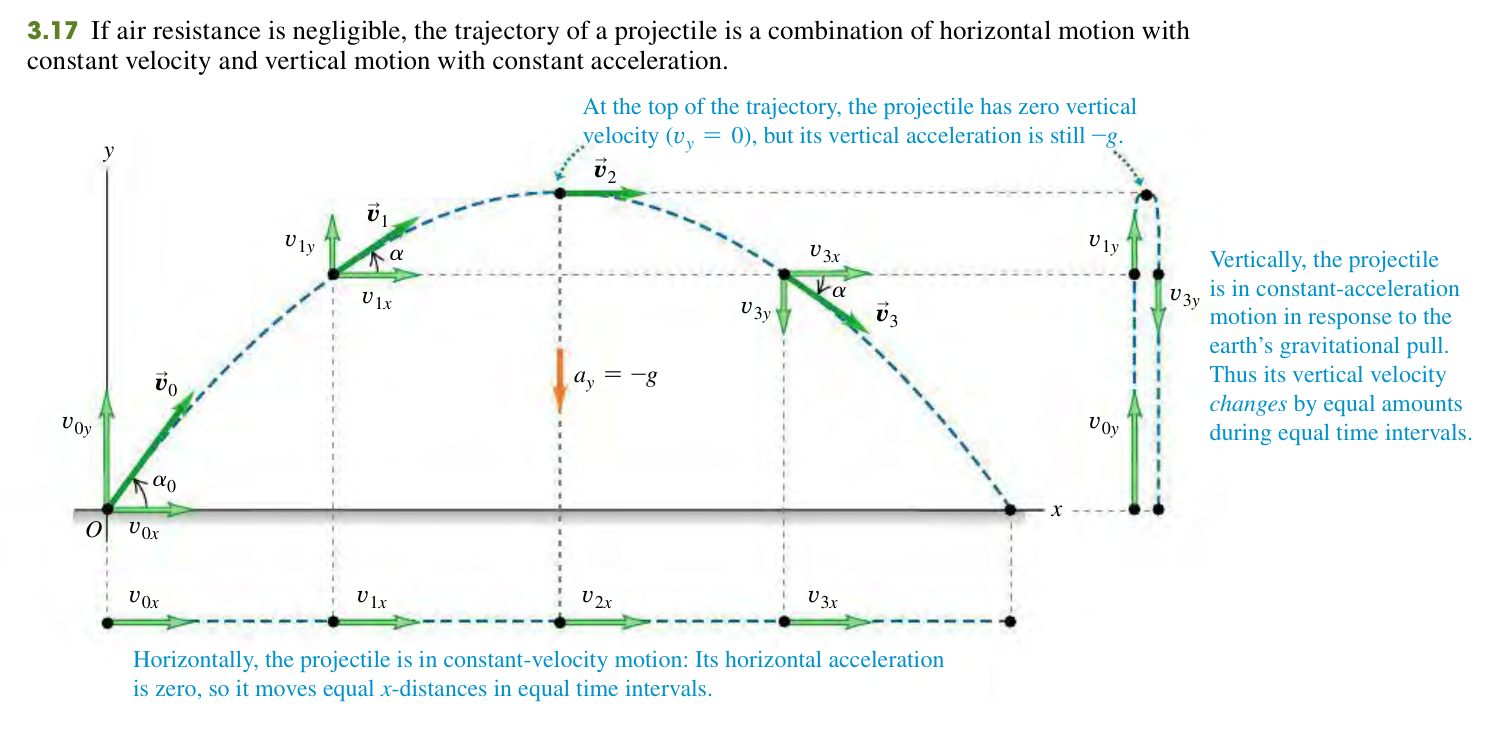
\includegraphics{images/parabolic_path.png}
\caption{parabolic}
\end{figure}

The key to analyzing projectile motion is treating the horizontal and
vertical coordinates as separate components. The horizontal and vertical
motions are independent, with the former having a constant velocity and
the latter experiencing a constant downward acceleration of -g (where g
is positive in the chosen coordinate system). By treating the motion as
a combination of the two components, we can express the projectile's
position, velocity, and acceleration as separate equations for the
horizontal and vertical motions.

This is an example of the independence of perpendicular motion. An
object dropped from rest will reach the ground at the same time as an
object thrown horizontally from the same height.

\begin{figure}
\centering
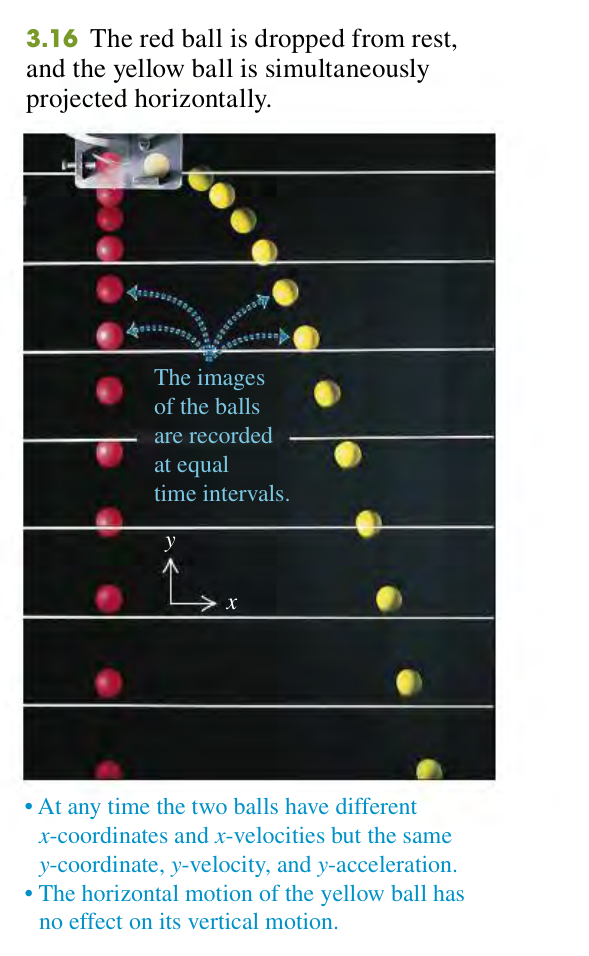
\includegraphics{images/independence.png}
\caption{independence}
\end{figure}

Since the acceleration is constant we use the kinematic equations. We
will start by setting up the kinematic equations and the dynamical
variables so the reader understands the splitting of components and also
the pattern in the equations themselves that will prove useful later.
Later on we will take a ``backwards'' approach and use Newton's law to
derive the kinematic equations and other equations we need.

\hypertarget{the-kinematic-equations}{%
\subsubsection{\texorpdfstring{\textbf{The Kinematic
Equations}}{The Kinematic Equations}}\label{the-kinematic-equations}}

In this case the acceleration is -g in the y-direction and 0 in the
x-direction. The kinematic equations in terms of x are:

\(x(t) = x_0 + v_{x0}t + \frac{1}{2}a_xt^2\)

\(v_x(t) = v_{x0} + a_xt\)

\(v_x^2 = v_{x0}^2 + 2a_x(x-x_0)\)

\(v_x = \frac{x-x_0}{t}\)

    \hypertarget{lets-break-down-each-equation.}{%
\paragraph{\texorpdfstring{\textbf{Let's break down each
equation.}}{Let's break down each equation.}}\label{lets-break-down-each-equation.}}

Due to the independence of perpendicular motion, changing components
simply requires changing the subscript and x to y.

\begin{enumerate}
\def\labelenumi{\arabic{enumi}.}
\tightlist
\item
  Displacement:

  \begin{itemize}
  \tightlist
  \item
    \(x(t) = x_0 + v_{x0}t + \frac{1}{2}a_xt^2\)
  \item
    This equation relates the displacement (x) of an object to its
    initial velocity (v\_i\_x), time (t), and acceleration (a\_x).
  \end{itemize}
\item
  Final Velocity:

  \begin{itemize}
  \tightlist
  \item
    \(v_x(t) = v_{x0} + a_xt\)
  \item
    This equation relates the final velocity (v\_f\_x) of an object to
    its initial velocity (v\_i\_x), time (t), and acceleration (a\_x).
  \end{itemize}
\item
  Velocity Squared:

  \begin{itemize}
  \tightlist
  \item
    \(v_x^2 = v_{x0}^2 + 2a_x(x-x_0)\)
  \item
    This equation calculates the velocity squared (v\_x\^{}2) of an
    object by adding the initial velocity squared (v\_i\_x\^{}2) to
    twice the acceleration (a\_x) multiplied by the displacement
    (x-x\_0).
  \end{itemize}
\item
  Velocity:

  \begin{itemize}
  \tightlist
  \item
    \(v_x = \frac{x-x_0}{t}\)
  \item
    This equation calculates the velocity (v\_x) of an object by
    dividing the displacement (x-x\_0) by the time (t) taken.
  \end{itemize}
\end{enumerate}

These equations are fundamental in analyzing the motion of objects under
constant acceleration. They allow us to determine various quantities
such as displacement, velocity, acceleration, and time in a given
scenario.

In this case, we are interested in the motion of a projectile. We can
use these equations to determine the projectile's position, velocity,
and acceleration in the x and y directions.

Appying the equations to our projectile motion scenario, we get the
following:

\begin{enumerate}
\def\labelenumi{\arabic{enumi}.}
\tightlist
\item
  Horizontal motion:

  \begin{itemize}
  \tightlist
  \item
    Displacement in the x-direction:

    \begin{itemize}
    \tightlist
    \item
      \(x = x_0 + v_{0x} t\)
    \end{itemize}
  \item
    Velocity in the x-direction:

    \begin{itemize}
    \tightlist
    \item
      \(v_x = v_{0x}\)
    \end{itemize}
  \item
    Acceleration in the x-direction:

    \begin{itemize}
    \tightlist
    \item
      \(a_x = 0\)
    \end{itemize}
  \end{itemize}
\item
  Vertical motion:

  \begin{itemize}
  \tightlist
  \item
    Displacement in the y-direction:

    \begin{itemize}
    \tightlist
    \item
      \(y = y_0 + v_{0y} t - \frac{1}{2} g t^2\)
    \end{itemize}
  \item
    Velocity in the y-direction:

    \begin{itemize}
    \tightlist
    \item
      \(v_y = v_{0y} - g t\)
    \end{itemize}
  \item
    Acceleration in the y-direction:

    \begin{itemize}
    \tightlist
    \item
      \(a_y = -g\)
    \end{itemize}
  \end{itemize}
\end{enumerate}

From these core kinematic equations we can derive other useful equations
for projectile motion.

    \hypertarget{maximum-height}{%
\paragraph{\texorpdfstring{\textbf{Maximum
height}}{Maximum height}}\label{maximum-height}}

The maximum height is reached when the vertical velocity is zero.
Therefore, we can set the vertical velocity to zero and solve for t.
This gives us the time at which the projectile reaches its maximum
height.

\(v_y = v_{0y} - g t\)

\(0 = v_{0y} - g t\)

\(t = \frac{v_{0y}}{g}\)

Substituting this value of t into the equation for vertical displacement
gives us the maximum height.

\(y = y_0 + v_{0y} \frac{v_{0y}}{g} - \frac{1}{2} g \frac{v_{0y}^2}{g^2}\)

\(y = y_0 + \frac{v_{0y}^2}{g} - \frac{v_{0y}^2}{2g}\)

\(y = y_0 + \frac{v_{0y}^2}{2g}\)

Therefore, the maximum height reached by the projectile is given by:

\(y_{max} = y_0 + \frac{1}{2} \frac{v_{0y}^2}{g}\)

    \hypertarget{time-of-flight}{%
\paragraph{\texorpdfstring{\textbf{Time of
Flight:}}{Time of Flight:}}\label{time-of-flight}}

The time of flight, T, is defined as the time taken by the projectile to
reach the ground. This time is given by:

\(T = \frac{2v₀ sin(θ)}{g}\)

where: - v₀ is the initial velocity of the projectile - θ is the launch
angle - g is the acceleration due to gravity

Deriving the time of flight is a simple matter of finding the time at
which the projectile hits the ground. This can be done by setting the
vertical displacement to zero and solving for t.

\(y = y₀ + v₀ sin(θ) t - \frac{1}{2} g t²\)

\(0 = y₀ + v₀ sin(θ) t - \frac{1}{2} g t²\)

\(0 = t (v₀ sin(θ) - \frac{1}{2} g t)\)

\(t = 0\)

\(v₀ sin(θ) - \frac{1}{2} g t = 0\)

\(t = \frac{2 v₀ sin(θ)}{g}\)

\(T = \frac{2 v₀ sin(θ)}{g}\)

    \hypertarget{range}{%
\paragraph{\texorpdfstring{\textbf{Range:}}{Range:}}\label{range}}

The range in projectile motion refers to the horizontal distance
traveled by the projectile before it lands back on the same level as its
initial launch point.

The range, R, in projectile motion is given by:

\(R = \frac{v₀² sin(2θ)}{g}\)

where: - v₀ is the initial velocity of the projectile - θ is the launch
angle - g is the acceleration due to gravity

The derivation for the range is as follows:

\(R = v₀ cos(θ) t\)

\(R = v₀ cos(θ) \frac{2v₀ sin(θ)}{g}\)

\(R = \frac{2v₀² sin(θ) cos(θ)}{g}\)

\(R = \frac{v₀² sin(2θ)}{g}\)

    \hypertarget{maximum-height-redux}{%
\paragraph{\texorpdfstring{\textbf{Maximum Height
Redux}}{Maximum Height Redux}}\label{maximum-height-redux}}

Now that we have an expression for t, we can simplify our previous
expression for maximum height even further.

\(H_{max} = \frac{v₀² sin²(θ)}{(2g)}\)

where: - v₀ is the initial velocity of the projectile - θ is the launch
angle - g is the acceleration due to gravity

The derivation for maximum height is as follows:

\(H_{max} = v₀ sin(θ) t - \frac{1}{2} g t²\)

\(H_{max} = v₀ sin(θ) \frac{2v₀ sin(θ)}{g} - \frac{1}{2} g (\frac{2v₀ sin(θ)}{g})²\)

\(H_{max} = \frac{2v₀² sin²(θ)}{g} - \frac{4v₀² sin²(θ)}{g}\)

\(H_{max} = \frac{v₀² sin²(θ)}{(2g)}\)

    \hypertarget{importance-of-numerical-simulations-in-studying-projectile-motion}{%
\subsubsection{Importance of numerical simulations in studying
projectile
motion}\label{importance-of-numerical-simulations-in-studying-projectile-motion}}

Projectile motion is often taught as a fundamental concept in physics
education to help students learn about motion and gravity. This involves
launching objects into the air and observing their curved paths, which
gravity influences solely. However, projectile motion can become more
complex when it comes to realistic calculations.

One of the main challenges with projectile motion is the absence of a
straightforward analytical solution. Projectile motion lacks a
closed-form solution Unlike other problems with precise equations
describing position, velocity, and acceleration as time functions. This
is due to the inclusion of air resistance, which significantly impacts
the object's trajectory.

When air resistance cannot be ignored, calculating the trajectory
becomes more challenging because the effects of air resistance are
velocity-dependent. As a result, the acceleration is no longer constant.

To accurately model and predict projectile motion, computer simulations
are essential. Simulations use numerical integration methods to solve
the equations of motion, accounting for gravity, air resistance, and
other relevant forces. Simulations provide a step-by-step approximation
of the projectile's motion by discretizing time and iteratively updating
the object's position and velocity.

Simulations have several advantages when dealing with the complexities
of realistic projectile motion. They allow for incorporating intricate
mathematical models that consider the changing effects of air resistance
as the object moves through the air. Additionally, simulations provide a
flexible framework for exploring different scenarios by adjusting launch
angles, initial velocities, and environmental conditions.

Visualizations provided by simulations enhance the understanding of
projectile behavior. Dynamic plots of trajectory, velocity, and other
relevant quantities over time show how factors like air resistance
impact the projectile's path. This visual feedback fosters a
comprehensive comprehension of the complex behavior exhibited by
projectiles.

Simulations can also encompass more complex scenarios involving multiple
projectiles or interactions with obstacles, allowing for exploring
various strategies, such as optimizing launch parameters to achieve
specific objectives like maximum range or height.

    \hypertarget{theoretical-framework}{%
\subsection{Theoretical Framework}\label{theoretical-framework}}

\hypertarget{overview-of-newtons-laws-of-motion}{%
\subsubsection{Overview of Newton's Laws of
Motion}\label{overview-of-newtons-laws-of-motion}}

Newton's laws of motion provide a fundamental framework for
understanding the motion of objects. These laws, formulated by Sir Isaac
Newton in the 17th century, describe the relationship between the motion
of an object and the forces acting upon it. The three laws are:

\begin{enumerate}
\def\labelenumi{\arabic{enumi}.}
\item
  \textbf{Newton's First Law (Law of Inertia):} An object at rest will
  remain at rest, and an object in motion will continue in motion with
  constant velocity unless acted upon by an external force.
\item
  \textbf{Newton's Second Law (Law of Acceleration):} The acceleration
  of an object is directly proportional to the net force applied to it
  and inversely proportional to its mass.
\item
  \textbf{Newton's Third Law (Law of Action-Reaction):} For every force
  there is an force paired with it that is equal in magnitude and
  opposite in direction.
\end{enumerate}

Understanding Newton's laws of motion is crucial for analyzing the
behavior of projectiles and predicting their trajectories under the
influence of external forces such as gravity and air resistance.

\hypertarget{introduction-to-numerical-integration-methods}{%
\subsubsection{Introduction to Numerical Integration
Methods}\label{introduction-to-numerical-integration-methods}}

Numerical integration methods play a vital role in simulating and
analyzing projectile motion. These methods provide a means to
approximate the behavior of objects by discretizing time and numerically
calculating their positions, velocities, and accelerations at discrete
time intervals.

\hypertarget{euler-method}{%
\paragraph{Euler Method}\label{euler-method}}

One commonly used numerical integration method is the Euler method. It
is a straightforward approach that approximates the derivative of a
function using finite differences. In the context of projectile motion,
the Euler method can be employed to numerically integrate the equations
of motion and determine the trajectory of the projectile.

The Euler method involves dividing the time interval into small steps
and updating the position and velocity of the projectile based on the
current values and the calculated acceleration at each time step. While
the Euler method is relatively simple to implement, it has some
limitations, such as accumulating error over long integration periods
and being sensitive to step size.

The mathematics behind the Euler method will be discussed in more detail
in the next section, where we dive into the math details.

\hypertarget{brief-mention-of-other-integration-methods}{%
\paragraph{Brief Mention of Other Integration
Methods}\label{brief-mention-of-other-integration-methods}}

In addition to the Euler method, various other numerical integration
methods exist, offering different levels of accuracy and stability. Some
commonly used integration methods in the context of projectile motion
include:

\begin{itemize}
\item
  \textbf{Runge-Kutta Methods:} These are a family of numerical
  integration methods that provide higher accuracy compared to the Euler
  method by considering multiple intermediate steps. The fourth-order
  Runge-Kutta (RK4) method is particularly popular for its balance
  between accuracy and computational efficiency.
\item
  \textbf{Verlet Integration:} Verlet integration is a symplectic
  integration method commonly used for simulating conservative systems.
  It can be advantageous in certain cases where energy conservation is
  important.
\item
  \textbf{Adaptive Integration Methods:} These methods dynamically
  adjust the step size during the integration process to maintain a
  desired level of accuracy. Adaptive integration can help mitigate
  error accumulation and improve the efficiency of simulations.
\end{itemize}

\hypertarget{calculating-projectile-motion}{%
\subsection{\texorpdfstring{\textbf{Calculating Projectile
Motion}}{Calculating Projectile Motion}}\label{calculating-projectile-motion}}

With the foundational material out of the way we can begin setting the
stage for our specific problem, and where the necessity of the
simulation will come into play.

To begin with, we will explore projectie motion without drag, introduce
retarding forces, adn then finally introduce drag.

\hypertarget{projectile-motion-without-drag}{%
\subsubsection{\texorpdfstring{\textbf{Projectile Motion Without
Drag}}{Projectile Motion Without Drag}}\label{projectile-motion-without-drag}}

\hypertarget{solving-newtons-laws}{%
\paragraph{\texorpdfstring{\textbf{Solving Newton's
Laws}}{Solving Newton's Laws}}\label{solving-newtons-laws}}

Newton's second law for projectile motion in two dimensions is as
follows:

\(\vec{F} = m \vec{a} = m \vec{g}\)

Using the independence of perpendicular motion, we split the forces into
x and y components. And since the only force acting on the projectile is
gravity, the x-direction will not have any resulting force.

\(F_x = m \ddot{x} = 0\)

\(F_x = m \ddot{y} = -mg\)

Where the constant of gravity is given to three significant figures:
\(g = 9.81 m/s^2\)

Reviewing the dynamical variables for our system we have the following:

\begin{longtable}[]{@{}
  >{\raggedright\arraybackslash}p{(\columnwidth - 4\tabcolsep) * \real{0.2787}}
  >{\raggedright\arraybackslash}p{(\columnwidth - 4\tabcolsep) * \real{0.3607}}
  >{\raggedright\arraybackslash}p{(\columnwidth - 4\tabcolsep) * \real{0.3607}}@{}}
\toprule\noalign{}
\begin{minipage}[b]{\linewidth}\raggedright
Dynamical Variable
\end{minipage} & \begin{minipage}[b]{\linewidth}\raggedright
X-Direction (Subscript)
\end{minipage} & \begin{minipage}[b]{\linewidth}\raggedright
Y-Direction (Subscript)
\end{minipage} \\
\midrule\noalign{}
\endhead
\bottomrule\noalign{}
\endlastfoot
Initial position & \(x_0\) & \(y_0\) \\
Final position & \(x\) & \(y\) \\
Initial velocity & \(v_{0x}\) & \(v_{0y}\) \\
Final velocity & \(v_x\) & \(v_y\) \\
Acceleration & \(a_x\) & \(a_y\) \\
Time & \(t\) & \(t\) \\
\end{longtable}

    \hypertarget{solving-for-position}{%
\paragraph{\texorpdfstring{\textbf{Solving For
Position}}{Solving For Position}}\label{solving-for-position}}

Given that x = y = 0 at t = 0, since the particie is at the origin at
this time. We can integrate the equations of motion to find the position
of the particle at any time t.

\(\ddot{x} = a_x = 0\)

\(\dot{x} = \int_{0}^{t} a_x dt = v_{0x} + C = v_0 cos\theta + C\)

\(x = \int_{0}^{t} v_x dt = v_{0x}t + C_1 = v_0 cos\theta t + C_1\)

Using the initial conditions we can solve for the constants of
integration. In this case, since x = 0 at t = 0, we have:

\$ x = v\_0 cos\theta (0) + C = 0\$

\(C = 0\)

So the final equation of motion for the x-direction is:

\$ x = v\_0 cos\theta t \$

The same process can be used to solve for the y-direction:

\(\ddot{y} = a_y = -g\)

\(\dot{y} = \int_{0}^{t} a_y dt = v_{0y} + C = v_0 sin\theta - gt + C\)

\(y = \int_{0}^{t} v_y dt = v_{0y}t + C_1 = v_0 sin\theta t - \frac{1}{2}gt^2 + C_1\)

Using the initial conditions we can solve for the constants of
integration. In this case, since y = 0 at t = 0, we have:

\(y = v_0 sin\theta (0) - \frac{1}{2}g(0)^2 + C = 0\)

\(C = 0\)

Just like before.

Moving forward, a similar process will be used to determine the
constants of integrations, and the details will be skipped for brevity.
The process of determining the constants of integration involves
examining the initial conditions of the system, and then solving for the
constants of integration that satisfy those conditions.

The final equation of motion for the y-direction is:

\(y = v_0 sin\theta t - \frac{1}{2}gt^2\)

    \hypertarget{solving-for-speed}{%
\paragraph{\texorpdfstring{\textbf{Solving For
Speed}}{Solving For Speed}}\label{solving-for-speed}}

The speed of the projectile can be found by taking the magnitude of the
velocity vector:

\$ v = \sqrt{v_x^2 + v_y^2} \$

In this case, we have solved for the velocity already in the x and y
directions, so we can substitute those equations into the speed
equation:

\$ v = \sqrt{(v_0 cos\theta)^2 + (v_0 sin\theta - gt)^2} \$

Working out the algebra we get:

\$ v = \sqrt{v_0^2 - 2v_0 sin\theta gt + g^2t^2} \$

\hypertarget{solving-for-the-magnitude-of-the-position-vector}{%
\paragraph{\texorpdfstring{\textbf{Solving For The Magnitude of the
Position
Vector}}{Solving For The Magnitude of the Position Vector}}\label{solving-for-the-magnitude-of-the-position-vector}}

The position vector is a vector that points from the origin to the
position of the particle as it changes. To find the distance from the
origin to the particle, we can take the magnitude of the position
vector:

\$ r = \sqrt{x^2 + y^2} \$

In this case, we have solved for the position already in the x and y
directions, so we can substitute those equations into the position
equation:

\$ r =
\sqrt{(v_0 cos\theta t)^2 + (v_0 sin\theta t - \frac{1}{2}gt^2)^2} \$

Working out the algebra we get:

\$ r = \sqrt{v_0^2t^2 - 2v_0 sin\theta t^3 + \frac{1}{4}g^2t^4} \$

\hypertarget{solving-for-maxiumum-range}{%
\paragraph{\texorpdfstring{\textbf{Solving For Maxiumum
Range}}{Solving For Maxiumum Range}}\label{solving-for-maxiumum-range}}

Finally we will get the maximum range equation. Following the same steps
as before we have:

\$ x = v\_0 cos\theta t \$

\$ x = v\_0 cos\theta \frac{2v_0 sin\theta}{g} \$

\$ x = \frac{2v_0^2 sin\theta cos\theta}{g} \$

And converting this into a double angle we get:

\$ x = \frac{v_0^2 sin(2\theta)}{g} \$

From this we also see tht the maximum range occurs when
\(sin(2\theta) = 1\), which occurs when \(\theta = 45^{\circ}\)

Lastly we will do the same but in the y-direction:

\$ y = v\_0 sin\theta t - \frac{1}{2}gt\^{}2 \$

\$ y = v\_0 sin\theta \frac{2v_0 sin\theta}{g} -
\frac{1}{2}g(\frac{2v_0 sin\theta}{g})\^{}2 \$

\$ y = \frac{2v_0^2 sin^2\theta}{g} - \frac{2v_0^2 sin^2\theta}{g} \$

\$ y = 0 \$

This quick calculation shows that the maximum range refers to the
distance traveled in the horizontal direction, as the vertical direction
ends up at the same height as it started.

    \hypertarget{retarding-forces-and-the-need-for-numerical-methods}{%
\subsubsection{\texorpdfstring{\textbf{Retarding Forces And The Need For
Numerical
Methods}}{Retarding Forces And The Need For Numerical Methods}}\label{retarding-forces-and-the-need-for-numerical-methods}}

    At this point, all the system's dynamical variables have been solved.
The equations following the model configurations provide all the
information about the system. Integrating air drag makes things
interesting, as it no longer allows for a closed-form equation solution.
Approximation methods become necessary in this case.

    \hypertarget{retarding-forces}{%
\paragraph{\texorpdfstring{\textbf{Retarding
Forces}}{Retarding Forces}}\label{retarding-forces}}

A retarding force is a force that acts in the opposite direction of the
motion of the particle. In the case of projectile motion the retarding
force is air drag.

But handling drag, or any other retarding force is the same as handling
multiple forces, the superposition principle applies. So we can add the
retarding force to the equation of motion:

\$ \sum \vec{F} = \vec{F_g} + \vec{F_r} = m\vec{g} + \vec{F_r}(v)\$

In this case the rearding force is a function of the velocity of the
particle. We usually aprooximate the retarding force as some power of
velocity. Keep in mind this by itself, is another approximation in our
model, and retarding forces are usually far more complicated.

Where this model is useful is where the speed doesn't vary greatly.

\hypertarget{the-power-law-approximation}{%
\subparagraph{\texorpdfstring{\textbf{The Power Law
Approximation}}{The Power Law Approximation}}\label{the-power-law-approximation}}

The power law approximation is a common approximation for retarding
forces. It is given by:

\$ \vec{F_r} = -kv\^{}n \$

Where k is the strength of the retarding force, and n is a power.

Where the velocity is less than 24 m/s \texttt{n} is taken to be 1, and
for velocities between 24 m/s and the speed of sound \texttt{n} is taken
to be 2.

\hypertarget{air-drag}{%
\subparagraph{\texorpdfstring{\textbf{Air
Drag}}{Air Drag}}\label{air-drag}}

Air resistance is called drag. It is a retarding force that is
proportional to the square of the velocity of the particle and points
opposite to the direction of motion.

Keep in mind we are only adding in one other force that would be acting
on an object undergoing projectile motion. There are also
non-conservative forces from;

\begin{itemize}
\tightlist
\item
  Lift - this is perpendicular to drag and is caused by the shape of the
  projectile
\item
  Spin from the projectile
\item
  Oscillation of the projectile
\end{itemize}

Also, the velocity usually doesn't point along the symmetry access of
the projectile.

So for our cases we will take the power of the retarding force to be 2.
From here we can integrate the retarding force into our previous
calculation, and see how it diverges.

    \hypertarget{adding-in-air-drag}{%
\subsubsection{Adding in air drag}\label{adding-in-air-drag}}

Compared to before Newotn's equations of motions for projectile motion
with air drag included are now:

\(F_x = m \ddot{x} = -km\dot{x}\)

\$F\_x = m \ddot{y} = - km\dot{y} -mg \$

And our initial conditions are:

\(x(t = 0) = 0 = y(t = 0)\)

\(\dot{x}(t = 0) = v_0 cos\theta \equiv U\)

\(\dot{y}(t = 0) = v_0 sin\theta \equiv V\)

In order to solve the force in the x direction we have to use separation
of variables:

\(\frac{d\dot{x}}{dt} = -k\dot{x}\)

\(\frac{d\dot{x}}{\dot{x}} = -kdt\)

\(\int_{U}^{\dot{x}} \frac{d\dot{x}}{\dot{x}} = -k\int_{0}^{t}dt\)

\(ln(\dot{x}) - ln(U) = -kt\)

\(ln(\frac{\dot{x}}{U}) = -kt\)

\(\frac{\dot{x}}{U} = e^{-kt}\)

\(\dot{x} = Ue^{-kt}\)

Now we can integrate this to get the position in the x direction:

\(\int_{0}^{x} dx = \int_{0}^{t} Ue^{-kt}dt\)

\(x = \frac{U}{k}(1 - e^{-kt})\)

Now we can solve for the force in the y direction:

\(\frac{d\dot{y}}{dt} = -k\dot{y} - g\)

\(\frac{d\dot{y}}{\dot{y} + \frac{g}{k}} = -kdt\)

\(\int_{V}^{\dot{y}} \frac{d\dot{y}}{\dot{y} + \frac{g}{k}} = -k\int_{0}^{t}dt\)

\(ln(\dot{y} + \frac{g}{k}) - ln(V + \frac{g}{k}) = -kt\)

\(\frac{\dot{y} + \frac{g}{k}}{V + \frac{g}{k}} = e^{-kt}\)

\(\dot{y} + \frac{g}{k} = (V + \frac{g}{k})e^{-kt}\)

\(\dot{y} = (V + \frac{g}{k})e^{-kt} - \frac{g}{k}\)

Now we can integrate this to get the position in the y direction:

\(\int_{0}^{y} dy = \int_{0}^{t} ((V + \frac{g}{k})e^{-kt} - \frac{g}{k})dt\)

\(y = \frac{V + \frac{g}{k}}{k}(1 - e^{-kt}) - \frac{g}{k}t\)

Our last equation is in place. Now in order to find the time T required
for the entire trajectory we need to find the time when y = 0 and t = T.
This is given by:

\(0 = \frac{V + \frac{g}{k}}{k}(1 - e^{-kT}) - \frac{g}{k}T\)

\(\frac{V + \frac{g}{k}}{k}(1 - e^{-kT}) = \frac{g}{k}T\)

\(T = \frac{kV + g}{gk}(1 - e^{-kT})\)

This is a transcendental equation and cannot be solved analytically. We
can solve it numerically however. Two methods that will be discussed are
the perturbation method, which we will use as a baseline, and the Euler
method, which is what is implemented in the simulation.

    \hypertarget{using-the-euler-method-to-solve-the-transcendental-equation-numerically}{%
\subsubsection{\texorpdfstring{\textbf{Using The Euler Method To Solve
The Transcendental Equation
Numerically}}{Using The Euler Method To Solve The Transcendental Equation Numerically}}\label{using-the-euler-method-to-solve-the-transcendental-equation-numerically}}

The first step to solving a differential equation using numerical
methods is to convert the differential equation into a difference
equation. A difference equation is an equation that relates the values
of a function to the previous values of the function.

The most straightforward difference equation is a first-order difference
equation, which the following initial value problem can represent:

\begin{verbatim}
dy/dt = f(t, y)
y(t = 0) = y_0
\end{verbatim}

Here, \texttt{t} represents the independent variable, \texttt{y}
represents the unknown function, and \texttt{f(t,\ y)} denotes the
derivative of \texttt{y} with respect to \texttt{t}.

The Euler Method is a first-order numerical approximation technique that
approximates the solution of the above difference equation. It involves
dividing the interval of interest into smaller subintervals and updating
the approximate values of \texttt{y} at each step using the following
equation:

\begin{verbatim}
y(t + Δt) = y(t) + Δt * f(t, y)
\end{verbatim}

Here, \texttt{Δt} represents the step size, \texttt{y(t)} is the
approximate value of \texttt{y} at time \texttt{t}, and
\texttt{y(t\ +\ Δt)} is the updated approximate value at
\texttt{t\ +\ Δt}.

The Euler Method is called a first-order method because it is accurate
to the first order in \texttt{Δt}.

    All the background mathematics have been laid out. From here the article
will describe the simulation.

    \hypertarget{simulation-setup}{%
\subsection{Simulation Setup}\label{simulation-setup}}

The simulation is written using Python and implements the VPython
framework for visualization. The code was originally visualized in
Glowscript, a website that allows the user to execute code with VPython
statements in it from the browser. It has since been moved to Jupyter
Notebook for presentation, but still running the program in Glowscript
provides the best experience.

In order to use VPython in a Jupyter Notebook the following import
statement is required:

    \begin{tcolorbox}[breakable, size=fbox, boxrule=1pt, pad at break*=1mm,colback=cellbackground, colframe=cellborder]
\prompt{In}{incolor}{ }{\boxspacing}
\begin{Verbatim}[commandchars=\\\{\}]
\PY{k+kn}{import} \PY{n+nn}{vpython} \PY{k+kn}{import} \PY{o}{*}
\end{Verbatim}
\end{tcolorbox}

    From here, the rest of the simulation code is straightforward. The
author wants to highlight specific parts of the code that are important
to the simulation.

The first is the timestep.

\hypertarget{timestep}{%
\paragraph{Timestep}\label{timestep}}

When using the Euler method for numerical integration, the choice of
timestep \texttt{(dt)} plays a crucial role in determining the accuracy
and stability of the results. The timestep represents the size of each
time increment used in the numerical approximation.

The Euler method approximates the solution of a differential equation by
updating the values of the dependent variable at discrete time intervals
based on the current values and the derivative. The update equation in
the Euler method is given by:

\begin{verbatim}
y(t + dt) = y(t) + dy/dt * dt
\end{verbatim}

The choice of timestep affects the accuracy and precision of the
numerical approximation. If the timestep is too large, the Euler method
may introduce significant errors in the solution. This is because the
method assumes the derivative is constant over the entire timestep,
which may not hold for rapidly changing functions or complex systems.

When the timestep is small, the Euler method provides a better
approximation by capturing finer details and reducing the truncation
error. Smaller timesteps allow for more frequent updates of the
dependent variable, resulting in a more accurate approximation of its
behavior.

For the simulation expressly, the timestep is set to 0.01. This is a
good value for the simulation because it is small enough to provide a
good approximation of the solution but not so small that it takes a long
time to run.

    \hypertarget{force-function}{%
\paragraph{Force Function}\label{force-function}}

Next up is the force function.

    Here is the version without drag.

    \begin{tcolorbox}[breakable, size=fbox, boxrule=1pt, pad at break*=1mm,colback=cellbackground, colframe=cellborder]
\prompt{In}{incolor}{ }{\boxspacing}
\begin{Verbatim}[commandchars=\\\{\}]
\PY{k}{def} \PY{n+nf}{Fnet}\PY{p}{(}\PY{p}{)}\PY{p}{:}

    \PY{n}{Fnetx} \PY{o}{=} \PY{l+m+mi}{0} 
    \PY{n}{Fnety} \PY{o}{=} \PY{o}{\PYZhy{}}\PY{n}{m}\PY{o}{*}\PY{n}{g} 
    \PY{n}{Fnetz} \PY{o}{=} \PY{l+m+mi}{0} 
    
    \PY{k}{return} \PY{n}{vector}\PY{p}{(}\PY{n}{Fnetx}\PY{p}{,} \PY{n}{Fnety}\PY{p}{,} \PY{n}{Fnetz}\PY{p}{)}
\end{Verbatim}
\end{tcolorbox}

    Here the only necessary information to calculate the force is the
graviational constant g, since the force is constant.

    Here is the version with drag.

    \begin{tcolorbox}[breakable, size=fbox, boxrule=1pt, pad at break*=1mm,colback=cellbackground, colframe=cellborder]
\prompt{In}{incolor}{ }{\boxspacing}
\begin{Verbatim}[commandchars=\\\{\}]
\PY{k}{def} \PY{n+nf}{Fnet}\PY{p}{(}\PY{n}{v}\PY{p}{)}\PY{p}{:} \PY{c+c1}{\PYZsh{} since we are calculating drag we need the velocity}

    \PY{n}{Fdrag\PYZus{}mag} \PY{o}{=} \PY{n}{m}\PY{o}{*}\PY{n}{v}\PY{o}{.}\PY{n}{mag} \PY{c+c1}{\PYZsh{} [N].}

    \PY{n}{vuv} \PY{o}{=} \PY{n}{v}\PY{o}{/}\PY{n}{v}\PY{o}{.}\PY{n}{mag} \PY{c+c1}{\PYZsh{}Calculate a unit vector in the direction of the velocity.}
    \PY{n}{Fnetx} \PY{o}{=} \PY{o}{\PYZhy{}}\PY{n}{vuv}\PY{o}{.}\PY{n}{x} \PY{o}{*} \PY{n}{Fdrag\PYZus{}mag} 
    \PY{n}{Fnety} \PY{o}{=} \PY{o}{\PYZhy{}}\PY{n}{m}\PY{o}{*}\PY{n}{g} \PY{o}{\PYZhy{}} \PY{n}{vuv}\PY{o}{.}\PY{n}{y} \PY{o}{*} \PY{n}{Fdrag\PYZus{}mag} 
    \PY{n}{Fnetz} \PY{o}{=} \PY{o}{\PYZhy{}}\PY{n}{vuv}\PY{o}{.}\PY{n}{z} \PY{o}{*} \PY{n}{Fdrag\PYZus{}mag} 
    
    \PY{k}{return} \PY{n}{vector}\PY{p}{(}\PY{n}{Fnetx}\PY{p}{,} \PY{n}{Fnety}\PY{p}{,} \PY{n}{Fnetz}\PY{p}{)}
\end{Verbatim}
\end{tcolorbox}

    Here the calculation becomes more involved. Since drag depends on the
projectile's velocity, we have to pass velocity in as a function
argument. Then the unit vector in the velocity direction is calculated,
the magnitude of the drag using the power law approximation, and then
the two are multiplied by each other to get the drag force vector.

Since the vector must point in the opposite direction of the velocity,
we multiply the drag force vector by -1. Then the function returns the
resultant force as a vector.

    \hypertarget{numerical-loop}{%
\paragraph{Numerical Loop}\label{numerical-loop}}

Lastly we have the numerical loop. This is where the Euler method is
implemented. The loop is shown below:

    \begin{tcolorbox}[breakable, size=fbox, boxrule=1pt, pad at break*=1mm,colback=cellbackground, colframe=cellborder]
\prompt{In}{incolor}{ }{\boxspacing}
\begin{Verbatim}[commandchars=\\\{\}]
\PY{k}{while} \PY{n}{r}\PY{o}{.}\PY{n}{y} \PY{o}{\PYZgt{}}\PY{o}{=} \PY{o}{\PYZhy{}}\PY{l+m+mf}{0.1}\PY{p}{:} \PY{c+c1}{\PYZsh{} Stop the simulation when the projectile hits the ground.}
    \PY{n}{ball}\PY{o}{.}\PY{n}{pos} \PY{o}{=} \PY{n}{r} \PY{c+c1}{\PYZsh{} update the position of the projectile with every iteration of the loop}

    \PY{c+c1}{\PYZsh{} plots the position of the projectile as the time changes}
    \PY{n}{plot\PYZus{}x}\PY{o}{.}\PY{n}{plot}\PY{p}{(}\PY{n}{pos}\PY{o}{=}\PY{p}{(}\PY{n}{t}\PY{p}{,}\PY{n}{r}\PY{o}{.}\PY{n}{x}\PY{p}{)}\PY{p}{)}
    \PY{n}{plot\PYZus{}y}\PY{o}{.}\PY{n}{plot}\PY{p}{(}\PY{n}{pos}\PY{o}{=}\PY{p}{(}\PY{n}{t}\PY{p}{,}\PY{n}{r}\PY{o}{.}\PY{n}{y}\PY{p}{)}\PY{p}{)}
    \PY{n}{plot\PYZus{}z}\PY{o}{.}\PY{n}{plot}\PY{p}{(}\PY{n}{pos}\PY{o}{=}\PY{p}{(}\PY{n}{t}\PY{p}{,}\PY{n}{r}\PY{o}{.}\PY{n}{z}\PY{p}{)}\PY{p}{)}
    
    \PY{c+c1}{\PYZsh{} Plots the velocity of the projectile as the time changes.}
    \PY{n}{plot\PYZus{}vx}\PY{o}{.}\PY{n}{plot}\PY{p}{(}\PY{n}{pos}\PY{o}{=}\PY{p}{(}\PY{n}{t}\PY{p}{,}\PY{n}{v}\PY{o}{.}\PY{n}{x}\PY{p}{)}\PY{p}{)} 
    \PY{n}{plot\PYZus{}vy}\PY{o}{.}\PY{n}{plot}\PY{p}{(}\PY{n}{pos}\PY{o}{=}\PY{p}{(}\PY{n}{t}\PY{p}{,}\PY{n}{v}\PY{o}{.}\PY{n}{y}\PY{p}{)}\PY{p}{)}
    \PY{n}{plot\PYZus{}vz}\PY{o}{.}\PY{n}{plot}\PY{p}{(}\PY{n}{pos}\PY{o}{=}\PY{p}{(}\PY{n}{t}\PY{p}{,}\PY{n}{v}\PY{o}{.}\PY{n}{z}\PY{p}{)}\PY{p}{)}
    
    \PY{n}{T} \PY{o}{=} \PY{p}{(}\PY{l+m+mf}{0.5}\PY{p}{)}\PY{o}{*}\PY{n}{m}\PY{o}{*}\PY{n}{v}\PY{o}{.}\PY{n}{mag}\PY{o}{*}\PY{o}{*}\PY{l+m+mi}{2}
    \PY{n}{U} \PY{o}{=} \PY{n}{m}\PY{o}{*}\PY{n}{g}\PY{o}{*}\PY{n}{r}\PY{o}{.}\PY{n}{y}
    \PY{c+c1}{\PYZsh{} Plots the energy of the projectile as the time changes.}
    \PY{n}{plot\PYZus{}T}\PY{o}{.}\PY{n}{plot}\PY{p}{(}\PY{n}{pos}\PY{o}{=}\PY{p}{(}\PY{n}{t}\PY{p}{,}\PY{n}{T}\PY{p}{)}\PY{p}{)}
    \PY{n}{plot\PYZus{}U}\PY{o}{.}\PY{n}{plot}\PY{p}{(}\PY{n}{pos}\PY{o}{=}\PY{p}{(}\PY{n}{t}\PY{p}{,}\PY{n}{U}\PY{p}{)}\PY{p}{)}
    \PY{n}{plot\PYZus{}H}\PY{o}{.}\PY{n}{plot}\PY{p}{(}\PY{n}{pos}\PY{o}{=}\PY{p}{(}\PY{n}{t}\PY{p}{,}\PY{n}{U}\PY{o}{+}\PY{n}{T}\PY{p}{)}\PY{p}{)}

    \PY{c+c1}{\PYZsh{} Report information about projectile }
    \PY{k}{if}\PY{p}{(}\PY{n}{v}\PY{o}{.}\PY{n}{y} \PY{o}{\PYZlt{}} \PY{l+m+mf}{0.1} \PY{o+ow}{and} \PY{n}{v}\PY{o}{.}\PY{n}{y} \PY{o}{\PYZgt{}} \PY{o}{\PYZhy{}}\PY{l+m+mf}{0.1}\PY{p}{)}\PY{p}{:}
        \PY{n+nb}{print}\PY{p}{(}\PY{l+s+s1}{\PYZsq{}}\PY{l+s+s1}{Max Height: t = }\PY{l+s+s1}{\PYZsq{}}\PY{p}{,}\PY{n}{t}\PY{p}{,}\PY{l+s+s1}{\PYZsq{}}\PY{l+s+s1}{s | }\PY{l+s+s1}{\PYZsq{}}\PY{p}{,}\PY{l+s+s1}{\PYZsq{}}\PY{l+s+s1}{vy = }\PY{l+s+s1}{\PYZsq{}}\PY{p}{,} \PY{n}{v}\PY{o}{.}\PY{n}{y} \PY{p}{,}\PY{l+s+s1}{\PYZsq{}}\PY{l+s+s1}{m/s | y = }\PY{l+s+s1}{\PYZsq{}}\PY{p}{,} \PY{n}{r}\PY{o}{.}\PY{n}{y} \PY{p}{,}\PY{l+s+s1}{\PYZsq{}}\PY{l+s+s1}{m}\PY{l+s+s1}{\PYZsq{}}\PY{p}{)}
    \PY{k}{if}\PY{p}{(}\PY{n}{r}\PY{o}{.}\PY{n}{y} \PY{o}{\PYZlt{}} \PY{l+m+mf}{0.1} \PY{o+ow}{and} \PY{n}{r}\PY{o}{.}\PY{n}{y} \PY{o}{\PYZgt{}} \PY{o}{\PYZhy{}}\PY{l+m+mf}{0.1}\PY{p}{)}\PY{p}{:}
        \PY{n+nb}{print}\PY{p}{(}\PY{l+s+s1}{\PYZsq{}}\PY{l+s+s1}{Time to ground: t = }\PY{l+s+s1}{\PYZsq{}} \PY{p}{,} \PY{n}{t} \PY{p}{,} \PY{l+s+s1}{\PYZsq{}}\PY{l+s+s1}{s | y = }\PY{l+s+s1}{\PYZsq{}} \PY{p}{,} \PY{n}{r}\PY{o}{.}\PY{n}{y} \PY{p}{,} \PY{l+s+s1}{\PYZsq{}}\PY{l+s+s1}{m | x = }\PY{l+s+s1}{\PYZsq{}}\PY{p}{,} \PY{n}{r}\PY{o}{.}\PY{n}{x} \PY{p}{,}\PY{l+s+s1}{\PYZsq{}}\PY{l+s+s1}{ m}\PY{l+s+s1}{\PYZsq{}}\PY{p}{)}
        
    \PY{c+c1}{\PYZsh{} Use Newton\PYZsq{}s 2nd Law to update the ball\PYZsq{}s position and velocity.}
    \PY{n}{t} \PY{o}{=} \PY{n}{t} \PY{o}{+} \PY{n}{dt} 
    \PY{n}{f} \PY{o}{=} \PY{n}{Fnet}\PY{p}{(}\PY{n}{v}\PY{p}{)}
    \PY{n}{a} \PY{o}{=} \PY{n}{f}\PY{o}{/}\PY{n}{m} 
    \PY{n}{v} \PY{o}{=} \PY{n}{v} \PY{o}{+} \PY{n}{a}\PY{o}{*}\PY{n}{dt} 
    \PY{k}{if} \PY{n}{v}\PY{o}{.}\PY{n}{mag} \PY{o}{\PYZgt{}} \PY{l+m+mi}{24}\PY{p}{:}
        \PY{c+c1}{\PYZsh{} This check is used to make sure the velocity does not exceed 24 m/s}
        \PY{c+c1}{\PYZsh{} If it does, the power used must change from 1 to 2}
        \PY{n+nb}{print}\PY{p}{(}\PY{l+s+s2}{\PYZdq{}}\PY{l+s+s2}{velocity above 24 m/s}\PY{l+s+s2}{\PYZdq{}}\PY{p}{)}
    \PY{n}{r} \PY{o}{=} \PY{n}{r} \PY{o}{+} \PY{n}{v}\PY{o}{*}\PY{n}{dt} 
 
    \PY{n}{sleep}\PY{p}{(}\PY{n}{dt}\PY{p}{)}
\end{Verbatim}
\end{tcolorbox}

    Notice that we calculate the acceleration using the force function and
then use it to update the velocity and position before starting the loop
again.

    \hypertarget{visualization-and-interpretation-of-results}{%
\subsection{Visualization And Interpretation Of
Results}\label{visualization-and-interpretation-of-results}}

\hypertarget{no-drag}{%
\subsubsection{No Drag}\label{no-drag}}

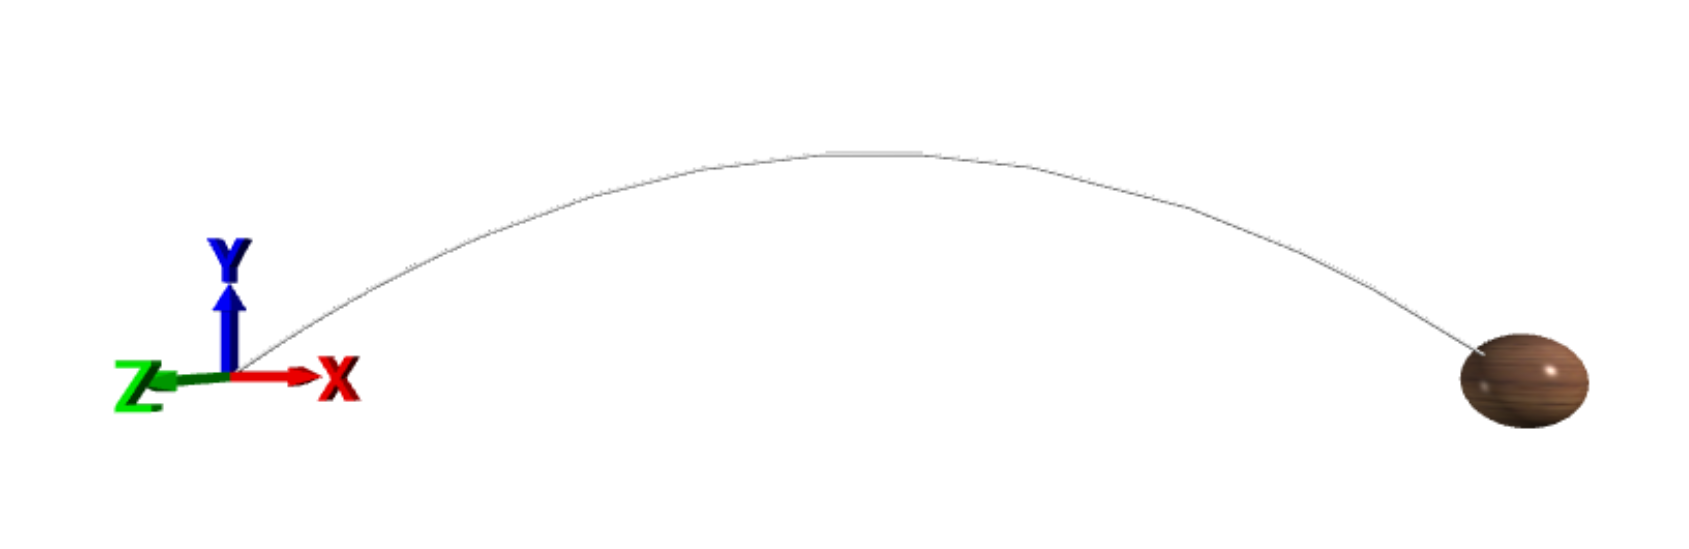
\includegraphics{images/no_drag/vis.png}
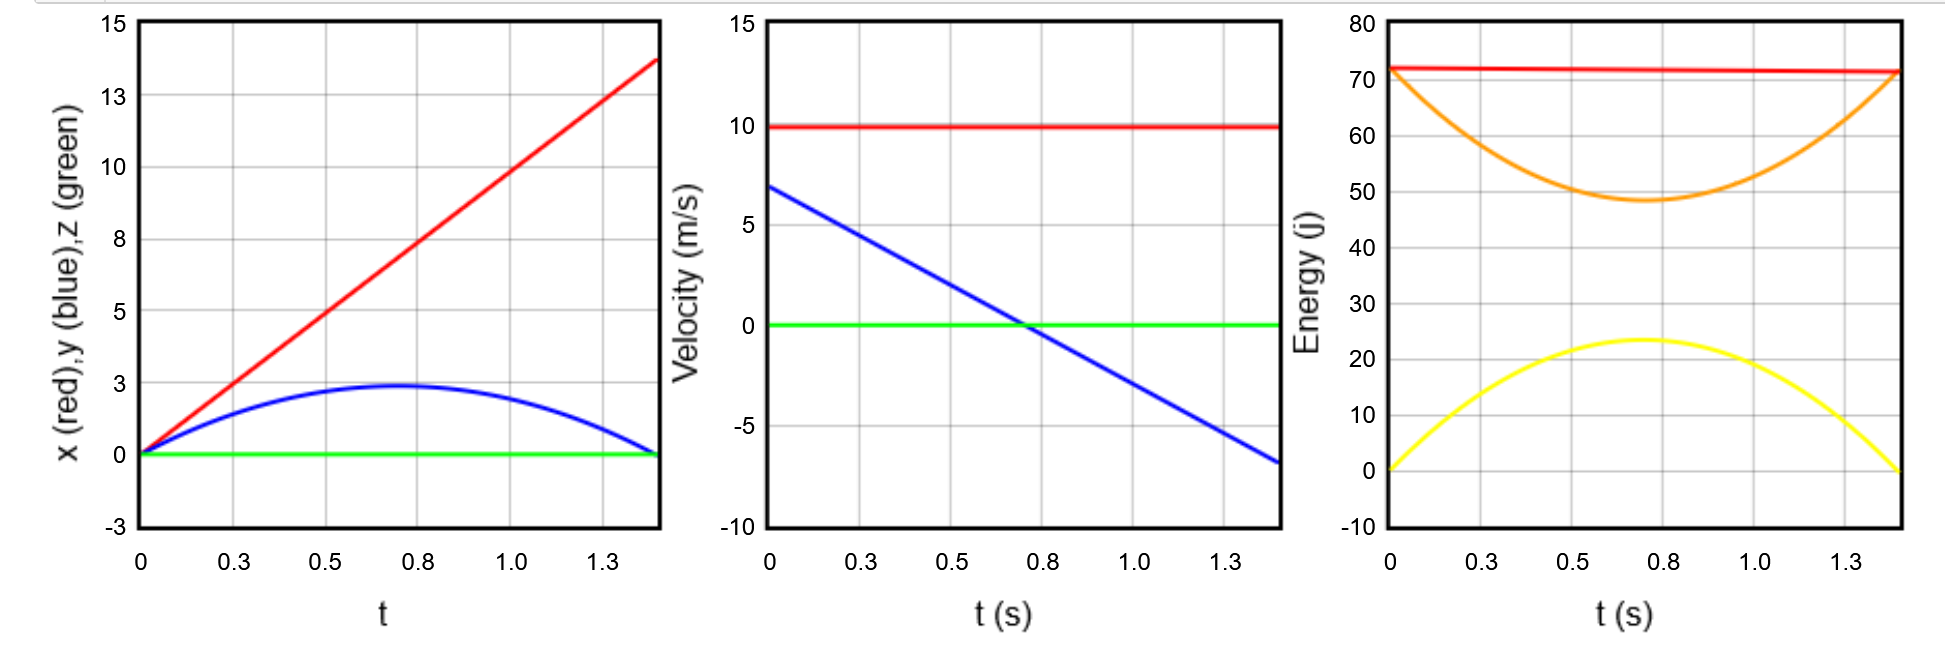
\includegraphics{images/no_drag/graph.png}
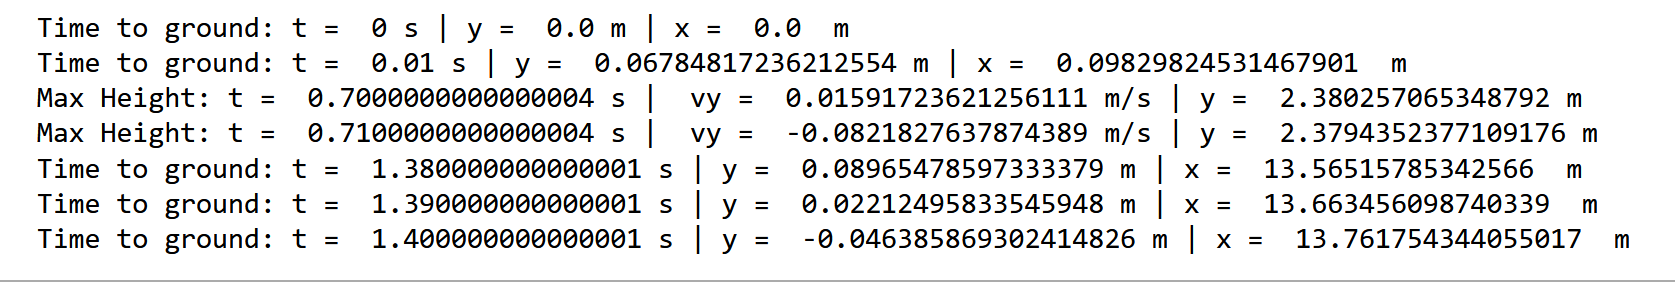
\includegraphics{images/no_drag/output.png}

From here, we can see that the energy changes from kinetic to potential
energy, then back to kinetic energy. The energy of the system as a whole
remains constant since there is no non-conservative work.

    \hypertarget{drag}{%
\subsubsection{Drag}\label{drag}}

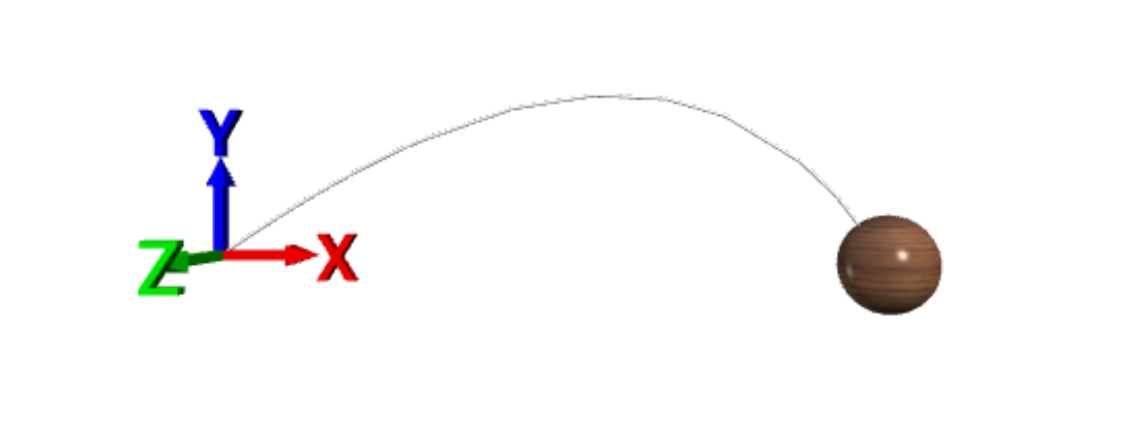
\includegraphics{images/drag/vis.png}
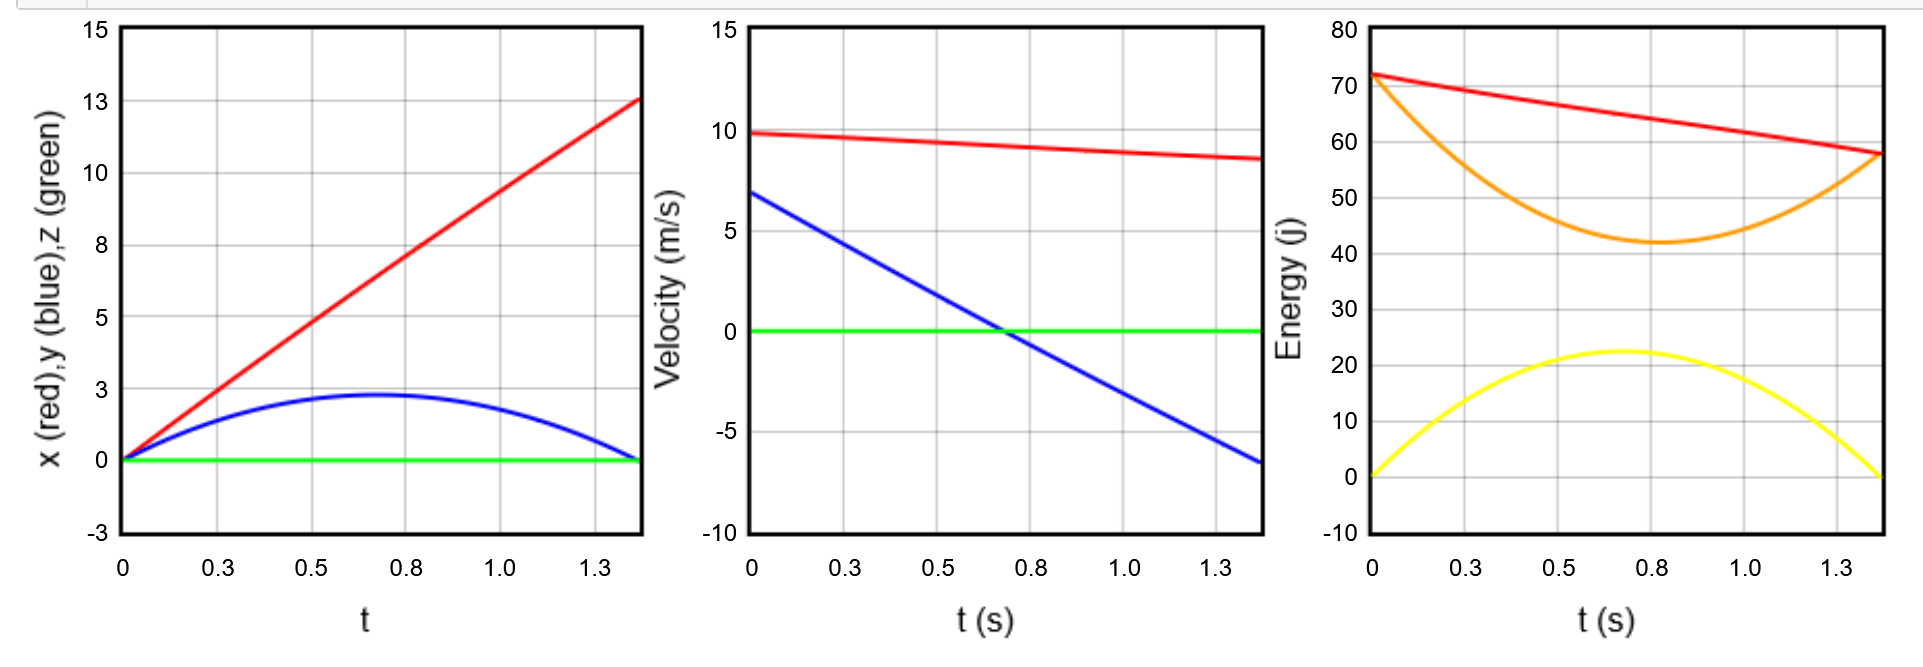
\includegraphics{images/drag/graphs.png}
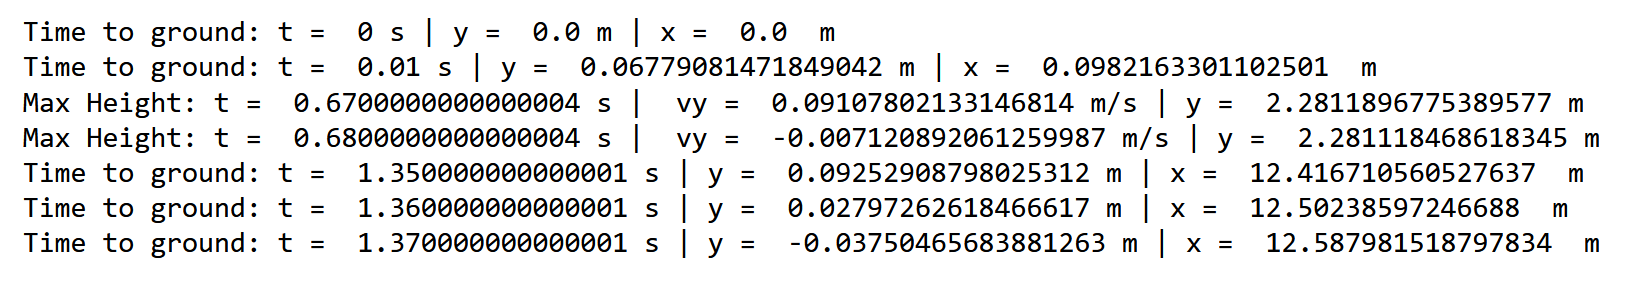
\includegraphics{images/drag/output.png}

One noticeable contrast between the two simulations is that the
projectile with drag has a significantly reduced range compared to the
one without. This is because the drag force is directly proportional to
the square of the velocity. Therefore, as the velocity increases
linearly, the drag force increases quadratically. This results in the
projectile losing its speed at a higher rate than the one without drag.

One notable distinction is that the system's energy is no longer
consistent due to non-conservative work. The drag force is responsible
for this non-conservative work, resulting in a gradual decrease in the
system's energy over time.

    \hypertarget{conclusion}{%
\subsection{Conclusion}\label{conclusion}}

    In conclusion, the Euler method is a straightforward and effective way
to solve differential equations numerically. It is straightforward to
implement and can solve various differential equations. It is also
straightforward to implement in a simulation.

By visualizing the two situations and comparing them, we gain valuable
insights into the physical situation of projectile motion. We can
immediately see a difference both in energy and range. Remember that the
Euler method is not the most accurate for solving differential
equations. Many other methods are more accurate and can solve more
complex differential equations. However, the Euler method is a good
starting point and can be used to gain a basic understanding of the
situation.

The primary thing to remember is that the projectile motion of actual
physical objects is much more complicated than the simple model
presented here, even with the drag taken into account and turning the
model into one that can no longer be solved analytically.

In reality, many other forces are acting on the projectile. We need to
add these forces to the simulation to obtain a more accurate projectile
motion model. However, we can take this simulation as a starting point
and build upon it to create a more accurate model.

    \hypertarget{references}{%
\subsection{References}\label{references}}

\begin{itemize}
\tightlist
\item
  Holley, Adam. ``Computational Physics.'' PHYS 4130. Tennessee
  Technological University, Fall 2022.
\item
  LibreTexts. ``Projectile Motion.'' Accessed June 10, 2023.
  https://phys.libretexts.org/Bookshelves/University\_Physics/Book\%3A\_Physics\_(Boundless)/3\%3A\_Two-Dimensional\_Kinematics/3.3\%3A\_Projectile\_Motion.
\item
  Chabay, Ruth, and Bruce Sherwood. ``GlowScript and Jupyter: VPython in
  a Browser (Vpython.Org),'' n.d.
\item
  Physics LibreTexts. ``3.3: Projectile Motion,'' April 12, 2018.
  https://phys.libretexts.org/Bookshelves/University\_Physics/Book\%3A\_Physics\_(Boundless)/3\%3A\_Two-Dimensional\_Kinematics/3.3\%3A\_Projectile\_Motion.
\item
  Thornton, Stephen T., and Jerry B. Marion. Classical Dynamics of
  Particles and Systems. 5th ed.~Belmont, CA: Brooks/Cole, 2004.
\item
  ``Web VPython.'' Accessed June 11, 2023. https://www.glowscript.org/.
\item
  Young, Hugh D., Roger A. Freedman, and Hugh D. Young. University
  Physics with Modern Physics. 15th edition. Hoboken, N.J: Pearson
  Higher Education, 2020.
\end{itemize}


    % Add a bibliography block to the postdoc
    
    
    
\end{document}
